%\documentclass[a4paper,10pt,draft,oneside,openbib,openright]{report}
\documentclass[a4paper,10pt,oneside,openright,openbib]{report}

\usepackage[utf8]{inputenc}
\usepackage[american]{babel}
\usepackage[T1]{fontenc}
%\usepackage[dvips,pdftex]{graphicx}
% only for DRAFT purposes
\usepackage[dvips]{graphicx}
\usepackage{makeidx}
\usepackage{pst-all}
\usepackage{subfigure}

\usepackage{ulem}

\usepackage{lastpage}
\usepackage{verbatim}
\usepackage{multirow}
\usepackage{tikz}
\usepackage{wrapfig}
\usepackage[nonumberlist, toc, section]{glossaries}
\usepackage{listings}
\usepackage{multicol}

\usepackage[light]{draftcopy}
%\usepackage[dvips,pdftex]{hyperref}
%
\usepackage{hyperref}
\hypersetup{colorlinks, 
	   citecolor=black,
	   filecolor=black,
	   linkcolor=black,
	   urlcolor=black,
	   bookmarksopen=true,
%	   pdftex}
}


\author{
%Armin Bauer <abauer@>\\ % TODO: ask for permission
Daniel Gollub <dgollub@suse.de>\\
}

\title{\huge{OpenSync}\\\large{A Synchronization Framework}}

\date{\today}


\begin{document}


\maketitle

\begin{quote}
Copyright \copyright{}  2008  Daniel Gollub.
Permission is granted to copy, distribute and/or modify this document
under the terms of the GNU Free Documentation License, Version 1.2
or any later version published by the Free Software Foundation;
with no Invariant Sections, no Front-Cover Texts, and no Back-Cover Texts.
A copy of the license is included in the section entitled ``GNU
Free Documentation License''. 
\end{quote}

\vfill
\begin{center}
(This page is \textbf{not} kept intentionally blank.)
\end{center}
\vfill

\tableofcontents

\newpage

%Abstract
\chapter*{Abstract}
\addcontentsline{toc}{subsection}{Abstract}
This document is a very detailed and technical paper about the OpenSync 
Framework, which gives a brief introduction about what the powerful OpenSync 
Framework provides and could be used for. It also covers lots of internal 
information for (ongoing) OpenSync developers. As well as for OpenSync Plugin 
and/or Frontend authors.\\
\\
Enjoy \& Don't forget to have fun!


%Introduction
\chapter{Introduction}
\label{chap:intro}
OpenSync is intended to be an universal Synchronization Framework, not limited to
a platform or desktop nor to PIM!

\section{History}
MultiSync, started by Bo Lincoln, was intended to synchronize various mobiles,
PDAs and PIM applications. MultiSync was a GTK application and provided
support for different PIM applications and devices by providing plugins.
The primary focus of MultiSync was to synchronize just PIM data (contacts, 
appointments, notes). Unfortunately this approach was fixed to a single UI and 
limited to PIM synchronization. Development branch MultiSync 0.9x was 
intended fix those needs.\\
\\
Early in 2005, Armin Bauer started refactoring the MultiSync project and
separated the UI code from MultiSync and the Plugin interface and
Synchronization logic. The result of his work is the most powerful and
flexible Synchronization Framework, known today as OpenSync.
\section{Big Picture}
OpenSync is intended to provide a low-level synchronization API for all kinds of 
data.
\\
\begin{figure}
 \centering
 % \includegraphics[bb=0 0 222 140,scale=0.5]{bigpicture}
 % bigpicture.png: 222x140 pixel, 72dpi, 7.83x4.94 cm, bb=0 0 222 140
 \caption{OpenSync}
 \label{fig:bigpicture}
\end{figure}


\section{Goals}
The goals of the OpenSync project are:

\begin{itemize}
 \item Reusabilty. OpenSync should be usable for all kinds of synchronization 
 applications
 \item Speed. Synchronization should be efficent and as fast as possible to give the
 user the best experience.
 \item Flexibility. Nobody can predict what will come next to synchronize after the
 G- \& iPhone, so OpenSync has to be designed and built as flexible and modular 
 as possible.
 \item Integrity. Data MUST never be lost or malformed, no matter what happens. 
 Data loss is just a no go!
 \item Portability. OpenSync should run on as many platforms as possible as 
 possible.
 \item Fun. The experience of using and developing OpenSync MUST be fun! You 
 should not work on OpenSync if you're unhappy :)
\end{itemize}
Not all of the mentioned goals are achieved yet, but OpenSync tries to get 
close as possible over time.

\section{Who should read this document?}
This Document is intended for everyone who is interested in a Open Source 
Synchronization solution. This is not a HowTo, Tutorial or Guide on how to use 
OpenSync. It is a detailed introduction of the OpenSync framework. No (high) 
programming skills/experince are required for this document.

\section{How should this document be read?}
Some chapter are very detailed about internal technial stuff, which is mainly 
intended for developers or people who are interested in how OpenSync works. Those
chapters could be safely skipped if someone isn't interested in touching the
internals of the OpenSync Framework. Such sections are marked with a little hint.

\section{Is this the most recent version of this paper?}
Maybe not, OpenSync is in a very early stage of development and lots of stuff
might changed within the last weeks. If in doubt, you might compare your version 
with the one from:\\
\\
\hyperref[http://www.opensync.org/download/LATEST-WHITEPAPER]{http://www.opensync.org/download/LATEST-WHITEPAPER}\\
\\
This paper was created on: \today


%Synchronization
\chapter{Synchronization}
This chapter give a brief introduction of synchronization basics as well as how
OpenSync works and handles real life synchronization issues.\\
\\
Different synchronization techniques used nowadays, which have some of the
following tasks in common:
\begin{itemize}
 \item Connect
 \item Get changes
 \item Conflict resolution
 \item Multiply changes
 \item Commit changes
 \item Disconnect
\end{itemize}
Those tasks are in common for synchronization technique/protocol, but differ in
detail to fit the needs for different circumstances to meet the best efficiency.
Such circumstances could be:
\begin{itemize}
 \item Number of synchronization parties. If the number of synchronization
 parties is two, then multiplying of changes is just simple duplication of the
 change.
 \item Unidirectional/Bidirectional synchronization. On unidirectional
 synchronization no conflict resolution required for two parties.
 \item Resource. Depending of the type of data resource further work is required
 to get changes. Is the resource able to tell which data changed since the last
 synchronization, by its own? Or is further help/facility required to detect
 which data changed since the last sync. Example: file systems, databases,
 stacked data in a single file, ...
 \item Type of data. Is the data in a consistent format and supported by all
 parties? File synchronization. Is the data not consistent and contains unique
 information which doesn't allow to do a binary compare? Weak compare? Is 
 conversion to a common format for different parties required?
 \item Protocol. Does the protocol require to read only the latest changes or 
 all at once? Does the protocol support single commits or only all at once 
 (batch commit)?
 \item Transport. Are various transport layer involved? Does it require to
 connect and disconnect in a specified way? Limited bandwidth? Example: 
 Bluetooth, USB, ...
\end{itemize}
You see, there lots of different circumstances which makes it quite complicated
to meet all the needs of different ways to synchronize and synchronization 
protocols.\\
This is also only the tip of the iceberg, since it describes only the
synchronization role of the ">Server"<. 

\section{Synchronization Role}
The term ">Server"< is quite confusing,
especially in the combination of a synchronization protocol which uses a
transport protocol based on the ">Client"<- and ">Server<"-Model. Most famous
example is ">SyncML"<, which support among others the HTTP and OBEX protocol as
transport. You might know ">HTTP Server"< like the Apache Webserver and ">HTTP
Client"< like the Firefox Webbrowser. In SyncML you can have for example (same 
for other transports supported by SyncML):
\begin{itemize}
\item HTTP Server transport and act as Synchronization Server
\item HTTP Client transport and act as Synchronization Server
\item HTTP Server transport and act as Synchronization Client
\item HTTP Client transport and act as Synchronization Client
\end{itemize}
OpenSync doesn't care much about Transport Server/Client role, this is
up to the Plugins. There is only a little detail which OpenSync have to care
about plugin when they're acting as the transport Server role, which is about
that the plugin has to be initialized all the time so the client can connect.
More about this in the Plugin chapter.\\
\\
Unfortunately OpenSync supports in version 0.40 only the Synchronization role
Server. The passive role as Synchronization Client isn't yet implemented, but is
on the top of the project agenda. The reason for this is that the current
implementation of synchronization tasks/steps mentioned above are currently
fixed. As Synchronization Client the order and number of this synchronization 
steps/tasks would differ to the Server role. More about this issue you can find
in the Framework Chapter in section Synchronization Role.

\section{Slow Sync}
Various Synchronization protocols are using so called ">Slow Sync"<
synchronization technique. This consists of two types of synchronizations, the
already mentioned ">Slow Sync"< and a regular Synchronization (sometimes called
">Fast Sync<"). The difference between the Slow and the regular (Fast) Sync is 
that the regular one only transfers changes since the last synchronization. 
This means on a regular synchronization not all entries have to be transfered, 
converted. This makes the synchronization quite efficient and very fast. The
so called ">Slow Sync"< requests intentionally all entries, which makes the
synchronization a bit slower. Additionally the Synchronization Framework has to
interpret every single entry/change as newly added, since the Framework vanished
in advance the entire mappings and has to compare every single reported entry
from each party and find the fitting counterpart. This and the combination of
transferring all entries makes the synchronization compared to the regular
(Fast) synchronization very slow. The ">Slow Sync"< is only used in certain
cases to avoid data inconsistence and to keep all the data in sync. ">Slow
Sync"< got emitted in following circumstances:
\begin{itemize}
\item First/Initial Synchronization
\item Party got reseted (same as first sync)
\item Party got synchronized in meanwhile within another environment 
\item After an aborted/failed synchronization
\end{itemize}
\section{Object Types}
The term ">Object Types"< is in OpenSync used to describe the type/category of 
data. Example for ">Object Types"< are Contacts, Events, Todos, Notes or plain 
Data (like the content of a file) and others. (It's not limited to PIM Data!). 
Those Object Types get separated processed, to make it configurable which 
Object Type should get synchronized. Example: Only synchronize contacts of the 
mobile, no events, todos nor notes.
\section{Formats}
The ability to synchronize different Parties which use different formats, makes
the OpenSync Framework to a very powerful Synchronization Framework. In OpenSync
each Format is associated with one Object Type (see previous chapter). This
Object Type as common denominator for different formats makes it possible to
determine a conversion path between different formats. The conversion path
consists of various format converters, which are provided by Format Plugins.
Example: Two parties should synchronize their contacts (the Object Type). Party
A stores the contacts as VCard 3.0 and Party B stores the contacts in some
Binary Format. To synchronize the VCard 3.0 and the Random Binary Contact Format
format plugins have to register those formats and provide converters. The
Plugins don't have to provide converters for every known Format, often a certain
amount of converters to common formats or a common denominator format is enough
to create a conversion path between VCard 3.0 to Binary Contact Format.
\section{Mappings}
If an entry got changed on one Party, the logical same entry has to be updated
on the other parties while synchronization. Often different parties use
different ids to identify their entries. So it's required to map the logical
same entries which each others native id. The combination of those different
entries on different parties are called ">Mappings"<. Those ">Mappings"< make it
possible to determine a conflict if mapped entries got changed on different
parties the same time in a different way.
\section{Conflicts}
So called ">Conflicts"< appear if at least two entries of the same mapping got
changed in a different way. No conflict appears if all entries of the mapping
changed the same way. Such conflicts have to be handled by the Synchronization
Framework to avoid data loss. There are several ways to solve such conflicts.
OpenSync provides several different for a proper conflict resolution without
gaining unintended loss of data. Following conflict resolution are supported by
the OpenSync Framework:

\begin{itemize}
\item Solve, means intentionally choosing one of the conflicting entries to
solve the conflict. The chosen one will be multiplied to all parties and will
overwrite the other conflicting changes. This also allows to configure in
advance who is the ">Winning"< Party, who's changes will always used as the 
solving change (">master change"<) for the conflict.
\item Duplicate, (intentionally) will duplicate all changed entries. 
\item Latest, using the latest changed entry of the conflicting entries. This is
only an conflict resolution option if all changes provide within their formats
enough information to determine which got most recently changed.
\item Ignoring, (temporarily) the conflict till the next synchronization.
Conflicting entries will be read and compared again by the OpenSync Framework on
the next synchronization. To avoid inconsistence and data loss. If the
entries/changes are equal on the next synchronization the conflict is solved as
well. (This conflict resolution requires that the protocol of all parties is
able to request single entries, without triggering a "Slow Sync".)
\end{itemize}
\section{Capabilities}
\section{Filter}
OpenSync provides initial code for filtering, but it's not yet usable within
OpenSync 0.40. Looking forward to OpenSync 0.41!


%Framework Architecture
\chapter{Framework Architecture}

\section{IPC}
Part of the OpenSync framework is an Interprocess Communication system to
communicate with the Plugins. To avoid confusion between the different process
types of Plugins, and to make the IPC independent of Plugins, the neutral terms
">Client"< and >"Client Proxy<" got introduced. The IPC is allows full duplex 
(bidirectional) communication between Client and Proxy. Independent of the 
process type of the Client. The frameworks allows to communicate between three 
different process types of Clients:
\begin{itemize}
\item Threaded via pipes (two pipes for full duplex/bidirectional ipc. See
pipe(7))
\item Forked via pipes (two pipes for full duplex/bidirectional ipc. See pipe(7))
\item External process via named pipes (FIFO)
\end{itemize}
This IPC also to send specific type of messages between the Client and the
Proxy. The Proxy takes care about timeout handling, if a client doesn't
response in time. This is only supported for messages which have a callback
function assigned. Such callbacks (command handler) get executed as soon if the
message reply by the Client is retrieved. On a timeout or error the callback
function got called with the custom error or timeout message.

\subsection{Client}
Clients handle all requests from the Proxy. Each request from the proxy gets
replied. Threaded and Forked clients get started by the Proxy. Most common use of
the Client is to call Plugin specific functions, requested with message send by
the Proxy. The client replies the result of the function calls with replying to
the messaged which requested the event.

\subsection{Proxy}
The Proxy handles all request to and from the Client. For each Client there is
one Proxy. The proxy got mainly used by the OpenSync framework engines to
communicate with the Plugin processes.

\subsection{Messaging Queues}
The communication between Client and Proxy is based on message queues. There are
two types of such Queues: Sender- and Receiver-Queue. The Queue object supports
(anonymous) pipes as well as named pipes (FIFO).\\
\\
Note: When using Queues along forked processes the read and write ends have to
be disconnected/closed for proper communication. See pipe(7).\\
\\
There is a specified set of Message Commands for simple communication between
Client and Proxy. For synchronized communication between Client and Proxy the
Client simply replies the Message Command from the Proxy, when Client executed
the requested command. If Client failed while executing the command, it has to
reply with an error reply. Synchronize communication requires that the caller
assign a message handler to the Message object, which got called when the
message got replied. This message handler should check carefully the received
replied message type, and handle provide proper error handling.\\
\\
For synchronized communication it's recommended to send message with a timeout
via the message queue. To avoid deadlocks when the counterpart fails to reply.
No timeout handling is needed for asynchronized communication without command
handler, since no reply is expected.\\
\\
Additional content of the message have to be marshaled/demarshaled, to make the
content usable even it's running in a different address space. (rough rule of 
thumb: everything which includes a pointers/memory addresses)

\section{Engines}
So called engines are the core of the entire framework and control the entire
sequence of every single step which is done during a synchronization. When the
engine got initialized it checks if a previous synchronization was unclean
(failed) and a slow sync is required. If the previous synchronization was
unclean or not could be only determined by engine itself if an group environment
is used. Beside the group environment it also initializes the plugin, format.
The engine isn't restricted to get called with a group environment, the group 
environment is only of optional use.\\
\\
If the group environment is used, the engine locks the group when the engine
gets initialized. If the group detects an unassigned lock the engine will
request while synchronization a slow sync.\\
\\
To determine a previous unclean synchronization without a group environment , 
it's up to OpenSync framework using program to provide facilities to store such 
information. If so, the engine MUST be set to trigger a slow sync, after it got 
initialized. When the engine got finalized or synchronized successful the slow 
sync engine status got reseted.\\
\\
With the engine initialization also the members of the group got initialized.
The member initialization creates for corresponding member plugin a Client Proxy
which got initialized and spawns the plugin. For more details check the IPC
section about the Proxy.\\
\\
After all members got initialized, the >"Object Engines<" for each enabled
Object Type got initialized. If no Object Type is enabled or discovered the
engine initialization aborts with an error. The engine needs at least one Object
Type to synchronize. Often this error appears if not all or none members got
discovered. See discover section of "Merging capabilities" for more details.

\subsection{Object Engine}
For each Object Type, which have to be synchronized, one Object Engine gets 
started by the (main) engine. If the engine detected that previous 
synchronization was unclean, each Object Engine get the slow sync flag set to 
perform a slow sync on the next sync. If the Object Engine got finalized or 
synchronized (successful or unsuccessful) the slow sync flag get reseted. If 
the synchronization failed, it's most likely that the (main) engine will set 
the slow sync flag again on the next synchronization.\\
\\
The Object Engines allows to perform actions only for a certain Object Type. For
example to request a slow sync only for specific Object Engines (this means also
for specific Object Types).\\
\\
The initialization of an Object Engine creates for each Client Proxy (read 
Members' Plugin) a Sink Engine, which maps each Client Proxy with an Object
Type. (More about the Sink Engine in the next section.)\\
\\
If a slow sync got set for the Object Engine, then all >"Mappings<" with the
Object Type of the Object Engine got deleted from the >"Mapping Table<". This is
done to avoid loss of the data inconsistence while performing a slow sync.\\
\\
If no slow sync got set for this Object Engine the >"Mapping Table<" got loaded
and creates for each Mapping a >"Mapping Engine<".

%TODO: Injecting ignored entries in mapping engine

%TODO


\subsection{Mapping Engine}
\subsection{Mapping Entry Engine}


\subsection{Sink Engine}
The Sink Engine currently doesn't consists of any logic. The only relation to
Engines of the Sink Engine object is, it maps all the already mentioned engines
together.\\
\\
The Sink Engine maps the Client Proxy and Object Engine together. With this 
combination the Sink Engine is able to handle Object Type specific (aka. 
ObjTypeSink) tasks. Additionally it contains of a list of Mapping Engines, 
which handle Object Type and Client related Mappings only.

\section{Merging Different Capabilities}
\subsection{Capabilities}
\subsection{Archive}
\subsection{Merger \& Demerger}
\section{Helpers}
\subsection{Anchor Table}
\subsection{Hash Table}
\subsection{Time Helper}
\section{Filter}
\subsection{Custom Fiter}


%Plugins
\chapter{Synchronization Plugins}
Synchronization Plugins are modules which provides access to a certain device,
application or protocol. All of those plugins provide independent of the
synchronized content/format or connection type, the same functions:
\begin{itemize}
\item initialize. This function parse the plugin configuration and initializes
the plugin. If the plugin acts as server, it also initializes this one and 
listen for incoming connections.
\item finalize. This function releases all gained memory by the plugin and stops
the listening server if present. 
\item discover. This function is intended to get called initially to gain
information about the target application, device or system. In detail it detects
all supported formats and individual capabilities of this format, if possible.
And basic information about the target application/device like version, vendor,
product, etc. ...
%\item usable. This function is intended to check if the target
%application/device is usable.
\end{itemize}

\begin{figure}
 \centering
 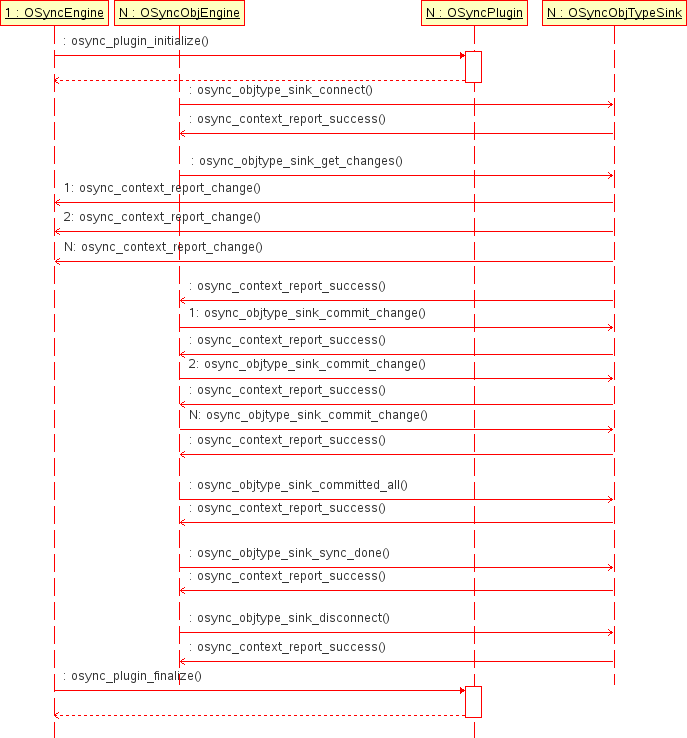
\includegraphics[bb=0 0 661 960, scale=0.60]{simple-sync-sequence}
 % simple-sync-sequence.png: 661x960 pixel, 72dpi, 23.32x33.87 cm, bb=0 0 661 960
 \caption{Plugin Synchronization Sequence}
 \label{fig:SimpleSyncSequence}
\end{figure}

Those function are called "Generic Functions" and MUST be implemented by 
plugin.

\section{Plugin module functions}
The plugin module functions are called once synchronously when the module
is loaded.
\subsection{get\_sync\_info}
This is the entry point for the plugin.  Once the plugin is loaded
\verb|get_sync_info| is called to determine the connectors provided by the
plugin. A single plugin may provide module may provide several connectors.  For
example the syncml plugin provides syncml-obex, syncml-http-client and
syncml-http-server connectors.

In this function a plugin must create an OSyncPlugin for each of the connectors
it provides.  The initialize, discover and finalize functions for each provided
conector must be set using the coressponding \verb|osync_plugin_set|
function. Each OSyncPlugin is added to the passed plugin environment using
\verb|osync_plugin_env_register_plugin|.

Return TRUE on success.  If an error occurs set OSyncError and return FALSE.
\section{Plugin specific functions}
These functions are called for a particular plugin that was registered in
\verb|get_sync_info|.
\subsection{Initialize}
The next call to the plugin will be to initialize a particular connector that
was registered in get\_sync\_info.  At this point the engine will have read the
plugin config which can be accessed using \verb|osync_plugin_info_get_config|

During this function the plugin should set itself up and register functions for each
objtype.

The passed OSyncPluginInfo contains a list of OSyncObjTypeSink.  Each of these
represents an objtype (e.g. contact, event) that the engine is capable of
syncing.  For each of these the plugin must:

Register Sink functions using \verb|osync_objtype_sink_set_xyz_func 
i.e. osync_objtype_sink_set_connect_func|

If a MainSink is needed (e.g. to connect to an interface that is shared between
several objtype sinks) it can be created and registered using:
\verb|osync_objtype_main_sink_new| \verb|osync_plugin_info_set_main_sink|

The function should return it's data cast to (void *) on success.  On failure
return NULL and set OSyncError to a user friendly explaination of the failure
cause.
\subsection{Discover}
In this function the plugin reports which objtype sinks are available, sets
version information and if requiring dynamically generated capabilities reports
them here.  Initialize will already have been called.

If an objtype can be syncronized then it should be set available using
\verb|osync_objtype_sink_set_available|.  Again the OSyncPluginInfo contains a
list of objtypes known to the engine.

There are two ways to describe the capabilities of a plugin: Dynamic and Static.
Not defining any capabilties WILL lead to data loss unless your plugin supports
all possible attributes.
\subsubsection{Static Capabilties}
Static capabilities are described in xml files shipped with a plugin.  A
descriptions.xml file links OSyncVersion properties to a particular capabilites
xml file. If no capabilities are set by the plugin in discover the engine will
use the version info to find the best matching capbilities.  If several
capabilities files match then the one with the ?highest/lowest? capability is
used.

\begin{verbatim}
Use the osync_verion_set functions as required.

	OSyncVersion *version = osync_version_new(error);
	osync_version_set_plugin(version, "pluginname");
	osync_version_set_modelversion(version, "version");
	osync_version_set_firmwareversion(version, "firmwareversion");
	osync_version_set_softwareversion(version, "softwareversion");
	osync_version_set_hardwareversion(version, "hardwareversion");
	osync_plugin_info_set_version(info, version);
\end{verbatim}

\subsubsection{Dynamic capabilities generation}
If the capabilities of a peer can only be known by querying it or can not be set using the
static capabilities method. The plugin must generate the capabilities.

Create new capabilities using:
\verb|osync_capabilities_new and osync_capability_new|
Add the capabilities to the plugin info using:
\verb|osync_plugin_info_set_capabilities|
\subsection{Finalize}
Clean up and free any allocated memory
%\subsection{Usable}
\section{Sink Functions}
All "Sink Functions" are called asynchronously, and must reply with OSyncContext functions.
 It's very important that the ">Sink Functions"< reply to the
request by the OpenSync Framework with the OSyncContext functions. Even on
error condition the Sink Function have to reply with a special OSyncContext
error function. Otherwise the OpenSync Framework will wait until the timeout for this
function call is reached before failing the function.

The Main Sink, which has no object type doesn't have any required Sink 
Functions. For Object Type Sinks the implementation of some Sink 
Functions required:

\begin{center}
% use packages: array
\begin{tabular}{ll}
\textbf{Function} & \textbf{Implementation} \\ 
Connect & Optional \\
Connect Done & Optional \\
Get Changes & Required \\ 
Commit & Required \\ 
Committed All & Optional (only available in combination with Commit)\\ 
Synchronization Done & Optional \\ 
Disconnect & Optional
\end{tabular}
\end{center}

The sink for which the sink function has been called is passed as the first parameter

\subsection{Connect}
The Connect function is available for all Object Type Sinks and could be used to
establish Object Type specific connection. If the connection establishment is an
Object Type neutral task (e.g. Bluetooth, USB, ...) and needs to be done only
once, only the Main Sink should be given a connect function. This avoids
problems with shared access to an interface, since a connect function would
otherwise be called for each Object Type for the same interface.

It is usual at this stage to compare the stored anchor with that from the peer
using \verb|osync_sink_state_equal|.  If the anchor has changed then the need for
a slow sync should be set using \verb|osync_context_report_slowsync|

This function MUST only establish a connection to the device or resource. After
the connection has been successfully established successful the plugin MUST
reply with \verb|osync_context_reply_success()|. On error the plugin replies
with a human-readable (aka. userfriendly) error message using
\verb|osync_context_reply_error()|.
\subsection{Connect Done}
Called after all peers have connected.  At this point the slow sync status of
all peers is known.  If your plugin must connect differently depending on the
group slow sync status then you may perform that connection here.
\subsection{Get Changes}
The Get Changes function gets called by the OpenSync Framework to request changes
since last synchronization or all entries of the Object Type specific resource.
The later case MUST be performed when a Slow Sync got requested by the OpenSync
Synchronization framework. The Slow Sync status of this Sink is passed as a osync_bool
slow_sync parameter. On a Slow Sync the 
Changetype (for all changes) is \verb|OSYNC_CHANGE_TYPE_ADDED|. On a regular 
(fast sync) synchronization it's up to the Get Changes function to determine 
the Changetype. Every change has to be reported with 
\verb|osync_context_report_change()|. On error the Sink Function must
reply with \verb|osync_context_report_error()| and stop/leave this 
function ASAP. If the protocol, application or device isn't able to report 
changed entries since last sync, the OpenSync Helper Hashtable should be used 
to determine the Changetype of the entry.
\subsection{Commit}
This function get called with a single OSyncChange object, which MUST be
committed to the application or device. If the commit failed the context MUST be
replied with \verb|osync_context_report_error()|. On success the context get
replied with \verb|osync_context_success()|. If Hashtable is already involved in
the Get Changes functions, then the Commit function should update the Hashtable
for the entries which get committed.
\subsection{Committed All}
This function is called after all entries have committed, even if error appeared
while committing.
\subsection{Synchronization Done}
This function is called only after a successful synchronization.  When using a
Hashtable \verb|osync_hashtable_save()| should be called to store the Hashtable
to disk.
\subsection{Disconnect}
This function MUST only handle the disconnect of the sink. Don't do further
cleanup here, the finalize function is intended for releasing memory and
cleanup. The disconnect function ???might be called even if the connect
function failed.
\section{Properties}
Each Synchronization Plugin has properties which get set within the
\verb|get_sync_info()| function. The properties are:

\begin{itemize}
\item Name, short name of the plugin should be less then 15 characters. This
name isn't visible to the user, at least not for rich OpenSync Frontends.
\item Longname, is the name of the plugin which is visible to the user in
rich OpenSync frontends. Should not be longer then 50 characters.
\item Description, about the Plugin visible to the end user in OpenSync
Frontends, and should additionally help to choose the right plugin.
\item Configuration Type, defines if the plugins needs any configuration or if
the configuration is optional or simply not needed.
\item Process Type, defines how the plugin get started: threaded, forked or by 
an external process.
\item Timeouts, for initialization, finalization and timeout can be configured
for the plugin needs. 
\end{itemize}

\subsection{Name}
The name of the plugin get defined like all plugin properties in
\verb|get_sync_info()| function with calling \verb|osync_plugin_set_name()|.
This name got used mostly for internal configuration and isn't visible to the 
user (at least not for rich OpenSync Frontend user). The name should be less
then 15 characters and should one word (no spaces). Example: ">palm-sync"<
\subsection{Longname}
The Longname of the plugin is the only name visible for  regular user to choose 
the correct plugin from a list of available plugins. Use the description field
to describe the plugin in more detail. Don't include the term ">Plugin"> in the
Longname. Example: ">Palm Device"<
\subsection{Description}
The description should additionaltly help the user to choose the correct plugin
if there are several plugins with similar names. Bad example: ">Plugin to sync 
your pda. Version 0.23. http://foo.edu/hacking/opensync"<. The term ">Plugin"< 
might confuse regular user, avoid it. If your plugin supports several different
devices don't list all known to work models, this might confuses people as well.
Again, don't list models! If your plugin is based on a synchronization 
implementation mention the name of protocol. No version numbers, no URLs and 
most user won't care about the authors name or E-Mail address.
\subsection{Plugin Timeouts}
The default plugin timeout should basically fit the need for all plugins. If
your plugin is known to be very slow you can change the timeout for this plugin
with following functions:
\begin{itemize}
\item \verb|osync_plugin_set_initliaze_timeout()|
\item \verb|osync_plugin_set_finalize_timeout()|
\item \verb|osync_plugin_set_discover_timeout()|
%\item \verb|osync_plugin_set_useable_timeout()|
\end{itemize}
The timeout unit is in seconds. It's possible to overwrite custom plugin timeout
with setting individual timeouts in the member configuration (syncmember.conf).
\subsection{Configuration Types}
If the plugin doesn't need any configuration by the user the plugin should the
configuration type to \verb|OSYNC_PLUGIN_NO_CONFIGURATION| with the
\verb|osync_plugin_set_config_type()| function. If the plugin don't need by
default a configuration but could be is additionally configurable the
configuration type should be set to \verb|OSYNC_PLUGIN_OPTIONAL_CONFIGURATION|. 
If the plugin can't perform without any configuration the type should be set
to\\ \verb|OSYNC_PLUGIN_NEEDS_CONFIGURATION| (set by default).
\subsection{Process Types}
The Process Type declares how a plugin get started. By default the plugin get
started by the OpenSync Framework within a thread (
\verb|OSYNC_START_TYPE_THREAD|). If the Plugin is known to conflict with the 
process mainloop of the OpenSync Framework, it's possible to run the plugin in 
a separated process by forking it. The forking is done by the OpenSync
Framework when the start type got set to \verb|OSYNC_START_TYPE_PROCESS|. If the
plugin has to access a not public interface to get access to the data resources
of an application it's possible to integrate the plugin within this application.
So the plugin is running all the time this application is running and can
communicate with the OpenSync Framework when the Process Type got set to 
\verb|OSYNC_START_TYPE_EXTERNAL|. The Process Type can be changed with the 
\verb|osync_plugin_set_start_type()| function. 
\section{Configuration}


%Format Plugins
\chapter{Format Plugins}
\section{Converter}
\section{Detectors}




%Environments
\chapter{Environments}
\section{Plugin Environment}
\section{Format Environment}
\section{Group Environment}



%Credits
\chapter{Credits}


\appendix

%Exampes
\chapter{Examples}
\section{Plugin}
\section{Format Plugin}
\section{User Interface}


%GNU FDL
%% This is set up to run with pdflatex.
%%---------The file header---------------------------------------------
%\documentclass[a4paper,12pt]{book}
%
%\usepackage[english]{babel} %language selection
%\selectlanguage{english}
%
%\pagenumbering{arabic}
%
%\usepackage{hyperref}
%\hypersetup{colorlinks, 
%	   citecolor=black,
%	   filecolor=black,
%	   linkcolor=black,
%	   urlcolor=black,
%	   bookmarksopen=true,
%	   pdftex}
%
%\hfuzz = .6pt % avoid black boxes
%	   
%\begin{document}
%%---------------------------------------------------------------------
\chapter{\rlap{GNU Free Documentation License}}
\phantomsection  % so hyperref creates bookmarks
\addcontentsline{toc}{chapter}{GNU Free Documentation License}
%\label{label_fdl}

 \begin{center}

       Version 1.2, November 2002


 Copyright \copyright{} 2000,2001,2002  Free Software Foundation, Inc.
 
 \bigskip
 
     51 Franklin St, Fifth Floor, Boston, MA  02110-1301  USA
  
 \bigskip
 
 Everyone is permitted to copy and distribute verbatim copies
 of this license document, but changing it is not allowed.
\end{center}


\begin{center}
{\bf\large Preamble}
\end{center}

The purpose of this License is to make a manual, textbook, or other
functional and useful document ``free'' in the sense of freedom: to
assure everyone the effective freedom to copy and redistribute it,
with or without modifying it, either commercially or noncommercially.
Secondarily, this License preserves for the author and publisher a way
to get credit for their work, while not being considered responsible
for modifications made by others.

This License is a kind of ``copyleft'', which means that derivative
works of the document must themselves be free in the same sense.  It
complements the GNU General Public License, which is a copyleft
license designed for free software.

We have designed this License in order to use it for manuals for free
software, because free software needs free documentation: a free
program should come with manuals providing the same freedoms that the
software does.  But this License is not limited to software manuals;
it can be used for any textual work, regardless of subject matter or
whether it is published as a printed book.  We recommend this License
principally for works whose purpose is instruction or reference.


\begin{center}
{\Large\bf 1. APPLICABILITY AND DEFINITIONS\par}
\phantomsection
%\addcontentsline{toc}{section}{1. APPLICABILITY AND DEFINITIONS}
\end{center}

This License applies to any manual or other work, in any medium, that
contains a notice placed by the copyright holder saying it can be
distributed under the terms of this License.  Such a notice grants a
world-wide, royalty-free license, unlimited in duration, to use that
work under the conditions stated herein.  The ``\textbf{Document}'', below,
refers to any such manual or work.  Any member of the public is a
licensee, and is addressed as ``\textbf{you}''.  You accept the license if you
copy, modify or distribute the work in a way requiring permission
under copyright law.

A ``\textbf{Modified Version}'' of the Document means any work containing the
Document or a portion of it, either copied verbatim, or with
modifications and/or translated into another language.

A ``\textbf{Secondary Section}'' is a named appendix or a front-matter section of
the Document that deals exclusively with the relationship of the
publishers or authors of the Document to the Document's overall subject
(or to related matters) and contains nothing that could fall directly
within that overall subject.  (Thus, if the Document is in part a
textbook of mathematics, a Secondary Section may not explain any
mathematics.)  The relationship could be a matter of historical
connection with the subject or with related matters, or of legal,
commercial, philosophical, ethical or political position regarding
them.

The ``\textbf{Invariant Sections}'' are certain Secondary Sections whose titles
are designated, as being those of Invariant Sections, in the notice
that says that the Document is released under this License.  If a
section does not fit the above definition of Secondary then it is not
allowed to be designated as Invariant.  The Document may contain zero
Invariant Sections.  If the Document does not identify any Invariant
Sections then there are none.

The ``\textbf{Cover Texts}'' are certain short passages of text that are listed,
as Front-Cover Texts or Back-Cover Texts, in the notice that says that
the Document is released under this License.  A Front-Cover Text may
be at most 5 words, and a Back-Cover Text may be at most 25 words.

A ``\textbf{Transparent}'' copy of the Document means a machine-readable copy,
represented in a format whose specification is available to the
general public, that is suitable for revising the document
straightforwardly with generic text editors or (for images composed of
pixels) generic paint programs or (for drawings) some widely available
drawing editor, and that is suitable for input to text formatters or
for automatic translation to a variety of formats suitable for input
to text formatters.  A copy made in an otherwise Transparent file
format whose markup, or absence of markup, has been arranged to thwart
or discourage subsequent modification by readers is not Transparent.
An image format is not Transparent if used for any substantial amount
of text.  A copy that is not ``Transparent'' is called ``\textbf{Opaque}''.

Examples of suitable formats for Transparent copies include plain
ASCII without markup, Texinfo input format, LaTeX input format, SGML
or XML using a publicly available DTD, and standard-conforming simple
HTML, PostScript or PDF designed for human modification.  Examples of
transparent image formats include PNG, XCF and JPG.  Opaque formats
include proprietary formats that can be read and edited only by
proprietary word processors, SGML or XML for which the DTD and/or
processing tools are not generally available, and the
machine-generated HTML, PostScript or PDF produced by some word
processors for output purposes only.

The ``\textbf{Title Page}'' means, for a printed book, the title page itself,
plus such following pages as are needed to hold, legibly, the material
this License requires to appear in the title page.  For works in
formats which do not have any title page as such, ``Title Page'' means
the text near the most prominent appearance of the work's title,
preceding the beginning of the body of the text.

A section ``\textbf{Entitled XYZ}'' means a named subunit of the Document whose
title either is precisely XYZ or contains XYZ in parentheses following
text that translates XYZ in another language.  (Here XYZ stands for a
specific section name mentioned below, such as ``\textbf{Acknowledgements}'',
``\textbf{Dedications}'', ``\textbf{Endorsements}'', or ``\textbf{History}''.)  
To ``\textbf{Preserve the Title}''
of such a section when you modify the Document means that it remains a
section ``Entitled XYZ'' according to this definition.

The Document may include Warranty Disclaimers next to the notice which
states that this License applies to the Document.  These Warranty
Disclaimers are considered to be included by reference in this
License, but only as regards disclaiming warranties: any other
implication that these Warranty Disclaimers may have is void and has
no effect on the meaning of this License.


\begin{center}
{\Large\bf 2. VERBATIM COPYING\par}
\phantomsection
%\addcontentsline{toc}{section}{2. VERBATIM COPYING}
\end{center}

You may copy and distribute the Document in any medium, either
commercially or noncommercially, provided that this License, the
copyright notices, and the license notice saying this License applies
to the Document are reproduced in all copies, and that you add no other
conditions whatsoever to those of this License.  You may not use
technical measures to obstruct or control the reading or further
copying of the copies you make or distribute.  However, you may accept
compensation in exchange for copies.  If you distribute a large enough
number of copies you must also follow the conditions in section~3.

You may also lend copies, under the same conditions stated above, and
you may publicly display copies.


\begin{center}
{\Large\bf 3. COPYING IN QUANTITY\par}
\phantomsection
%\addcontentsline{toc}{section}{3. COPYING IN QUANTITY}
\end{center}


If you publish printed copies (or copies in media that commonly have
printed covers) of the Document, numbering more than 100, and the
Document's license notice requires Cover Texts, you must enclose the
copies in covers that carry, clearly and legibly, all these Cover
Texts: Front-Cover Texts on the front cover, and Back-Cover Texts on
the back cover.  Both covers must also clearly and legibly identify
you as the publisher of these copies.  The front cover must present
the full title with all words of the title equally prominent and
visible.  You may add other material on the covers in addition.
Copying with changes limited to the covers, as long as they preserve
the title of the Document and satisfy these conditions, can be treated
as verbatim copying in other respects.

If the required texts for either cover are too voluminous to fit
legibly, you should put the first ones listed (as many as fit
reasonably) on the actual cover, and continue the rest onto adjacent
pages.

If you publish or distribute Opaque copies of the Document numbering
more than 100, you must either include a machine-readable Transparent
copy along with each Opaque copy, or state in or with each Opaque copy
a computer-network location from which the general network-using
public has access to download using public-standard network protocols
a complete Transparent copy of the Document, free of added material.
If you use the latter option, you must take reasonably prudent steps,
when you begin distribution of Opaque copies in quantity, to ensure
that this Transparent copy will remain thus accessible at the stated
location until at least one year after the last time you distribute an
Opaque copy (directly or through your agents or retailers) of that
edition to the public.

It is requested, but not required, that you contact the authors of the
Document well before redistributing any large number of copies, to give
them a chance to provide you with an updated version of the Document.


\begin{center}
{\Large\bf 4. MODIFICATIONS\par}
\phantomsection
%\addcontentsline{toc}{section}{4. MODIFICATIONS}
\end{center}

You may copy and distribute a Modified Version of the Document under
the conditions of sections 2 and 3 above, provided that you release
the Modified Version under precisely this License, with the Modified
Version filling the role of the Document, thus licensing distribution
and modification of the Modified Version to whoever possesses a copy
of it.  In addition, you must do these things in the Modified Version:

\begin{itemize}
\item[A.] 
   Use in the Title Page (and on the covers, if any) a title distinct
   from that of the Document, and from those of previous versions
   (which should, if there were any, be listed in the History section
   of the Document).  You may use the same title as a previous version
   if the original publisher of that version gives permission.
   
\item[B.]
   List on the Title Page, as authors, one or more persons or entities
   responsible for authorship of the modifications in the Modified
   Version, together with at least five of the principal authors of the
   Document (all of its principal authors, if it has fewer than five),
   unless they release you from this requirement.
   
\item[C.]
   State on the Title page the name of the publisher of the
   Modified Version, as the publisher.
   
\item[D.]
   Preserve all the copyright notices of the Document.
   
\item[E.]
   Add an appropriate copyright notice for your modifications
   adjacent to the other copyright notices.
   
\item[F.]
   Include, immediately after the copyright notices, a license notice
   giving the public permission to use the Modified Version under the
   terms of this License, in the form shown in the Addendum below.
   
\item[G.]
   Preserve in that license notice the full lists of Invariant Sections
   and required Cover Texts given in the Document's license notice.
   
\item[H.]
   Include an unaltered copy of this License.
   
\item[I.]
   Preserve the section Entitled ``History'', Preserve its Title, and add
   to it an item stating at least the title, year, new authors, and
   publisher of the Modified Version as given on the Title Page.  If
   there is no section Entitled ``History'' in the Document, create one
   stating the title, year, authors, and publisher of the Document as
   given on its Title Page, then add an item describing the Modified
   Version as stated in the previous sentence.
   
\item[J.]
   Preserve the network location, if any, given in the Document for
   public access to a Transparent copy of the Document, and likewise
   the network locations given in the Document for previous versions
   it was based on.  These may be placed in the ``History'' section.
   You may omit a network location for a work that was published at
   least four years before the Document itself, or if the original
   publisher of the version it refers to gives permission.
   
\item[K.]
   For any section Entitled ``Acknowledgements'' or ``Dedications'',
   Preserve the Title of the section, and preserve in the section all
   the substance and tone of each of the contributor acknowledgements
   and/or dedications given therein.
   
\item[L.]
   Preserve all the Invariant Sections of the Document,
   unaltered in their text and in their titles.  Section numbers
   or the equivalent are not considered part of the section titles.
   
\item[M.]
   Delete any section Entitled ``Endorsements''.  Such a section
   may not be included in the Modified Version.
   
\item[N.]
   Do not retitle any existing section to be Entitled ``Endorsements''
   or to conflict in title with any Invariant Section.
   
\item[O.]
   Preserve any Warranty Disclaimers.
\end{itemize}

If the Modified Version includes new front-matter sections or
appendices that qualify as Secondary Sections and contain no material
copied from the Document, you may at your option designate some or all
of these sections as invariant.  To do this, add their titles to the
list of Invariant Sections in the Modified Version's license notice.
These titles must be distinct from any other section titles.

You may add a section Entitled ``Endorsements'', provided it contains
nothing but endorsements of your Modified Version by various
parties--for example, statements of peer review or that the text has
been approved by an organization as the authoritative definition of a
standard.

You may add a passage of up to five words as a Front-Cover Text, and a
passage of up to 25 words as a Back-Cover Text, to the end of the list
of Cover Texts in the Modified Version.  Only one passage of
Front-Cover Text and one of Back-Cover Text may be added by (or
through arrangements made by) any one entity.  If the Document already
includes a cover text for the same cover, previously added by you or
by arrangement made by the same entity you are acting on behalf of,
you may not add another; but you may replace the old one, on explicit
permission from the previous publisher that added the old one.

The author(s) and publisher(s) of the Document do not by this License
give permission to use their names for publicity for or to assert or
imply endorsement of any Modified Version.


\begin{center}
{\Large\bf 5. COMBINING DOCUMENTS\par}
\phantomsection
%\addcontentsline{toc}{section}{5. COMBINING DOCUMENTS}
\end{center}


You may combine the Document with other documents released under this
License, under the terms defined in section~4 above for modified
versions, provided that you include in the combination all of the
Invariant Sections of all of the original documents, unmodified, and
list them all as Invariant Sections of your combined work in its
license notice, and that you preserve all their Warranty Disclaimers.

The combined work need only contain one copy of this License, and
multiple identical Invariant Sections may be replaced with a single
copy.  If there are multiple Invariant Sections with the same name but
different contents, make the title of each such section unique by
adding at the end of it, in parentheses, the name of the original
author or publisher of that section if known, or else a unique number.
Make the same adjustment to the section titles in the list of
Invariant Sections in the license notice of the combined work.

In the combination, you must combine any sections Entitled ``History''
in the various original documents, forming one section Entitled
``History''; likewise combine any sections Entitled ``Acknowledgements'',
and any sections Entitled ``Dedications''.  You must delete all sections
Entitled ``Endorsements''.

\begin{center}
{\Large\bf 6. COLLECTIONS OF DOCUMENTS\par}
\phantomsection
%\addcontentsline{toc}{section}{6. COLLECTIONS OF DOCUMENTS}
\end{center}

You may make a collection consisting of the Document and other documents
released under this License, and replace the individual copies of this
License in the various documents with a single copy that is included in
the collection, provided that you follow the rules of this License for
verbatim copying of each of the documents in all other respects.

You may extract a single document from such a collection, and distribute
it individually under this License, provided you insert a copy of this
License into the extracted document, and follow this License in all
other respects regarding verbatim copying of that document.


\begin{center}
{\Large\bf 7. AGGREGATION WITH INDEPENDENT WORKS\par}
\phantomsection
%\addcontentsline{toc}{section}{7. AGGREGATION WITH INDEPENDENT WORKS}
\end{center}


A compilation of the Document or its derivatives with other separate
and independent documents or works, in or on a volume of a storage or
distribution medium, is called an ``aggregate'' if the copyright
resulting from the compilation is not used to limit the legal rights
of the compilation's users beyond what the individual works permit.
When the Document is included in an aggregate, this License does not
apply to the other works in the aggregate which are not themselves
derivative works of the Document.

If the Cover Text requirement of section~3 is applicable to these
copies of the Document, then if the Document is less than one half of
the entire aggregate, the Document's Cover Texts may be placed on
covers that bracket the Document within the aggregate, or the
electronic equivalent of covers if the Document is in electronic form.
Otherwise they must appear on printed covers that bracket the whole
aggregate.


\begin{center}
{\Large\bf 8. TRANSLATION\par}
\phantomsection
%\addcontentsline{toc}{section}{8. TRANSLATION}
\end{center}


Translation is considered a kind of modification, so you may
distribute translations of the Document under the terms of section~4.
Replacing Invariant Sections with translations requires special
permission from their copyright holders, but you may include
translations of some or all Invariant Sections in addition to the
original versions of these Invariant Sections.  You may include a
translation of this License, and all the license notices in the
Document, and any Warranty Disclaimers, provided that you also include
the original English version of this License and the original versions
of those notices and disclaimers.  In case of a disagreement between
the translation and the original version of this License or a notice
or disclaimer, the original version will prevail.

If a section in the Document is Entitled ``Acknowledgements'',
``Dedications'', or ``History'', the requirement (section~4) to Preserve
its Title (section~1) will typically require changing the actual
title.


\begin{center}
{\Large\bf 9. TERMINATION\par}
\phantomsection
%\addcontentsline{toc}{section}{9. TERMINATION}
\end{center}


You may not copy, modify, sublicense, or distribute the Document except
as expressly provided for under this License.  Any other attempt to
copy, modify, sublicense or distribute the Document is void, and will
automatically terminate your rights under this License.  However,
parties who have received copies, or rights, from you under this
License will not have their licenses terminated so long as such
parties remain in full compliance.


\begin{center}
{\Large\bf 10. FUTURE REVISIONS OF THIS LICENSE\par}
\phantomsection
%\addcontentsline{toc}{section}{10. FUTURE REVISIONS OF THIS LICENSE}
\end{center}


The Free Software Foundation may publish new, revised versions
of the GNU Free Documentation License from time to time.  Such new
versions will be similar in spirit to the present version, but may
differ in detail to address new problems or concerns.  See
http://www.gnu.org/copyleft/.

Each version of the License is given a distinguishing version number.
If the Document specifies that a particular numbered version of this
License ``or any later version'' applies to it, you have the option of
following the terms and conditions either of that specified version or
of any later version that has been published (not as a draft) by the
Free Software Foundation.  If the Document does not specify a version
number of this License, you may choose any version ever published (not
as a draft) by the Free Software Foundation.


%\begin{center}
%{\Large\bf ADDENDUM: How to use this License for your documents\par}
%\phantomsection
%\addcontentsline{toc}{section}{ADDENDUM: How to use this License for your documents}
%\end{center}
%
%To use this License in a document you have written, include a copy of
%the License in the document and put the following copyright and
%license notices just after the title page:
%
%\bigskip
%\begin{quote}
%    Copyright \copyright{}  YEAR  YOUR NAME.
%    Permission is granted to copy, distribute and/or modify this document
%    under the terms of the GNU Free Documentation License, Version 1.2
%    or any later version published by the Free Software Foundation;
%    with no Invariant Sections, no Front-Cover Texts, and no Back-Cover Texts.
%    A copy of the license is included in the section entitled ``GNU
%    Free Documentation License''.
%\end{quote}
%\bigskip
%    
%If you have Invariant Sections, Front-Cover Texts and Back-Cover Texts,
%replace the ``with \dots\ Texts.'' line with this:
%
%\bigskip
%\begin{quote}
%    with the Invariant Sections being LIST THEIR TITLES, with the
%    Front-Cover Texts being LIST, and with the Back-Cover Texts being LIST.
%\end{quote}
%\bigskip
%    
%If you have Invariant Sections without Cover Texts, or some other
%combination of the three, merge those two alternatives to suit the
%situation.
%
%If your document contains nontrivial examples of program code, we
%recommend releasing these examples in parallel under your choice of
%free software license, such as the GNU General Public License,
%to permit their use in free software.

%---------------------------------------------------------------------
%\end{document}


\end{document}
